% !TEX TS-program = pdflatex
% !TEX encoding = UTF-8 Unicode

% This is a simple template for a LaTeX document using the "article" class.
% See "book", "report", "letter" for other types of document.

\documentclass[11pt]{article} % use larger type; default would be 10pt

\usepackage[utf8]{inputenc} % set input encoding (not needed with XeLaTeX)

%%% Examples of Article customizations
% These packages are optional, depending whether you want the features they provide.
% See the LaTeX Companion or other references for full information.

%%% PAGE DIMENSIONS
\usepackage{geometry} % to change the page dimensions
\geometry{letterpaper} % or letterpaper (US) or a5paper or....
\geometry{margin=1in} % for example, change the margins to 2 inches all round
% \geometry{landscape} % set up the page for landscape
%   read geometry.pdf for detailed page layout information

\usepackage{graphicx} % support the \includegraphics command and options
\usepackage{hyperref}

\usepackage[parfill]{parskip} % Activate to begin paragraphs with an empty line rather than an indent

%%% PACKAGES
%\usepackage{booktabs} % for much better looking tables
\usepackage{array} % for better arrays (eg matrices) in maths
%\usepackage{paralist} % very flexible & customisable lists (eg. enumerate/itemize, etc.)
\usepackage{verbatim} % adds environment for commenting out blocks of text & for better verbatim
%\usepackage{subfig} % make it possible to include more than one captioned figure/table in a single float
% These packages are all incorporated in the memoir class to one degree or another...

%%% HEADERS & FOOTERS
\usepackage{fancyhdr} % This should be set AFTER setting up the page geometry
\pagestyle{fancy} % options: empty , plain , fancy
\renewcommand{\headrulewidth}{0pt} % customise the layout...
\lhead{}\chead{}\rhead{}
\lfoot{}\cfoot{\thepage}\rfoot{}

%%% END Article customizations

%%% The "real" document content comes below...

\title{Introduction to Actuators}
\author{}
\date{} % Activate to display a given date or no date (if empty),
         % otherwise the current date is printed 

\begin{document}
\maketitle

%\begin{quote}
%Wise quote here.\\ \hbox{}\hfil -- {\em A Wise One}
%\end{quote}

\section*{Introduction}

In this lab, you’ll explore electromagnetism and some common actuators. You’ll build a simple electromagnet and see how electromagnetism can be used both for sensing and actuation. You will then implement some basic mechanical actuators, namely a solenoid and an RC servo.

\subsection*{Objectives}

Upon successful completion of this lab, the student will be able to:
\begin{itemize}
\item Describe how electromagnetism can be used to create mechanical motion,
\item Describe the operation of solenoids and RC servo motors,
\item Describe the operation and purpose of mechanical relays,
\item Implement driver circuits for solenoids, relays, and RC servo motors,
\item Describe how Hall effect sensors can be used to detect magnetic fields,
\item Implement a Hall effect sensor for detecting the presence of a magnet, and
\item Implement a hysteresis band for control.
\end{itemize}

There will be a quiz this coming week.

\section*{Preparation}
\subsection*{Background materials}

Review the following materials:
\begin{itemize}
\item {\bf Electromagnetism and solenoids.} Read the few pages posted on collab.
\item The \href{https://learn.sparkfun.com/tutorials/hobby-servo-tutorial}{\underline{SparkFun tutorial on RC servos}} is pretty good.
\item Refresh your memory of hysteresis from the reading on event-driven programming.
\end{itemize}

\section*{In lab}

\subsection*{Electromagnetism}

An electromagnet can be created by winding wire into a coil and passing current through it. By wrapping the wire around a ferromagnetic material (such as an ordinary iron nail), the magnetic field becomes more concentrated and amplified. When no external magnetic field is applied to a ferromagnetic material, the magnetic domains within the material are randomly oriented and cancel themselves out so that the material produces no net magnetic field. When an external magnetic field is applied, however, the magnetic domains within the material tend to line up with the external field. These internal magnetic domains then add to the external field and create a more powerful electromagnet.

In this part of the lab, you will explore a homemade electromagnet made by wrapping a nail with insulated wire. You’ll use this device not only to create a magnetic field (by passing current through the windings) but also to sense an external magnetic field passing near it.

%\subsection{Background}
%
%The three equations provided in Figure~\ref{fig:em.laws} can be used to model the properties of this simple electromagnet. The equation on the left predicts the magnitude of the magnetic field that is generated by a coil of wire that is wrapped around a core material and carries an electrical current. The middle equation is used to model the amount of force that an electromagnet can exert on an external ferromagnetic object when the flux path is closed, though in our case the flux path is not closed -- you’d need to bend the nail into an upside-down “U” shape so that the flux flowing from the magnet’s North pole to its South pole could flow in a loop directly through iron instead of through both iron and air. 
%
%\begin{figure}[htbp]
%\begin{center}
%\includegraphics[width=5.5in]{figures/em_laws}
%\caption{Equations used in modeling an electromagnet and magnetic pickup.}
%\label{fig:em.laws}
%\end{center}
%\end{figure}

\subsubsection*{Procedure}
\label{sec:electromagnet}

\begin{enumerate}
\item (This step has probably been done for you -- ask before you go and wind your own!) Construct a homemade electromagnet by wrapping wire around a nail or screw a few hundred times -- we have a drill that is good for speeding things up. Make sure to leave a few inches of wire on each end for connecting the electromagnet to jumper wires. 
\item (This step has probably been done for you!) Remove an inch or so of the insulating enamel from the ends of the magnet wire by sanding them with fine grit sandpaper or scraping them with a knife until the copper beneath the enamel is fully exposed. You can also use a lighter to burn the enamel off. 
\item Using alligator clips, connect your electromagnet to a bench-top power supply with the voltage set to 0V for now. The power supplies are convenient because they are easily adjustable and also show the amount of current being drawn, but {\bf be careful not to run too much current through the coil for too long -- it will get hot and burn you!} 
\item Slowly turn up the voltage supply and verify that your electromagnet works by picking up nails, screws, or other ferromagnetic objects. Observe the amount of current flowing through the circuit versus the apparent strength of the electromagnet as you adjust the voltage on the power supply. How are they related?
\end{enumerate}

Note that since you are picking up ferromagnetic pieces of metal, it does not matter which direction current is flowing through your electromagnet’s coil -- a north pole attracts a piece of iron just as well as a south pole does. If you were trying to attract (or repel) a permanent magnet with an electromagnet (which is how a typical DC motor works) the direction of current flowing through an electromagnet’s coil becomes very important because it determines the polarity of the electromagnet.

\subsection*{Sensing using EMF}

The simple device made by wrapping coils of wire around a ferromagnetic core can serve another useful purpose. Now that you have created an electromagnet by sending electrical current through your coil, you will do the exact opposite and pass a changing magnetic field near the coil to generate electricity within the coil. When an external magnetic field passes near a coil of wire, an electromotive force (EMF) induces a voltage within the coil.  In this experiment, you’ll only generate enough electricity to make a ‘blip’ on the oscilloscope, but this is the basic principle behind electric generators.

\subsubsection*{Procedure}

\begin{enumerate}
\item Disconnect your electromagnet from the power supply and connect it directly to CH1 on your oscilloscope. You’ll want to do this with breadboard and banana clips -- sticking the tiny wires in the oscilloscope connectors is not going to end well.
\item Take a magnet and pass it near the end of the electromagnet such that the N-S axis of the magnet is parallel to the nail. Observe what happens on the oscilloscope. (You should see a small voltage spike on the oscilloscope each time this happens.)
\item Experiment with passing the magnet at different speeds and distances from the pickup. Why do these affect the magnitude of the voltage spike? What could you do to amplify these signals?
\item Turn the magnet around and repeat the experiment. How is the oscilloscope capture different? Why?
\end{enumerate}

{\bf Show your working system to an instructor.}

\vspace{0.25in}
Instructor initials: \rule{2in}{0.4pt}
\vspace{0.25in}

\subsection*{Hall effect sensor}
%\label{sec:hall.effect}

A typical Hall effect sensor contains a small conductive plate (called a Hall plate) with a steady electrical current flowing across it. When an external magnetic field is applied perpendicularly to the plate, a Lorentz force deflects the electrons flowing through the plate. This causes more negative charges to be on one side of the plate, which creates a voltage potential across the plate. As the strength of the external magnetic field increases, the voltage potential across the plate increases proportionally. The \href{https://www.parallax.com/sites/default/files/downloads/605-00005-MLX90217-Datasheet.pdf}{\underline{Melexis 90127 Hall effect sensor}} that you will use here incorporates some extra circuitry that amplifies the signal to output either a digital \verb|HIGH| or \verb|LOW|. Fundamentally, what component do you think it uses to do this?

\begin{figure}[htbp]
\begin{center}
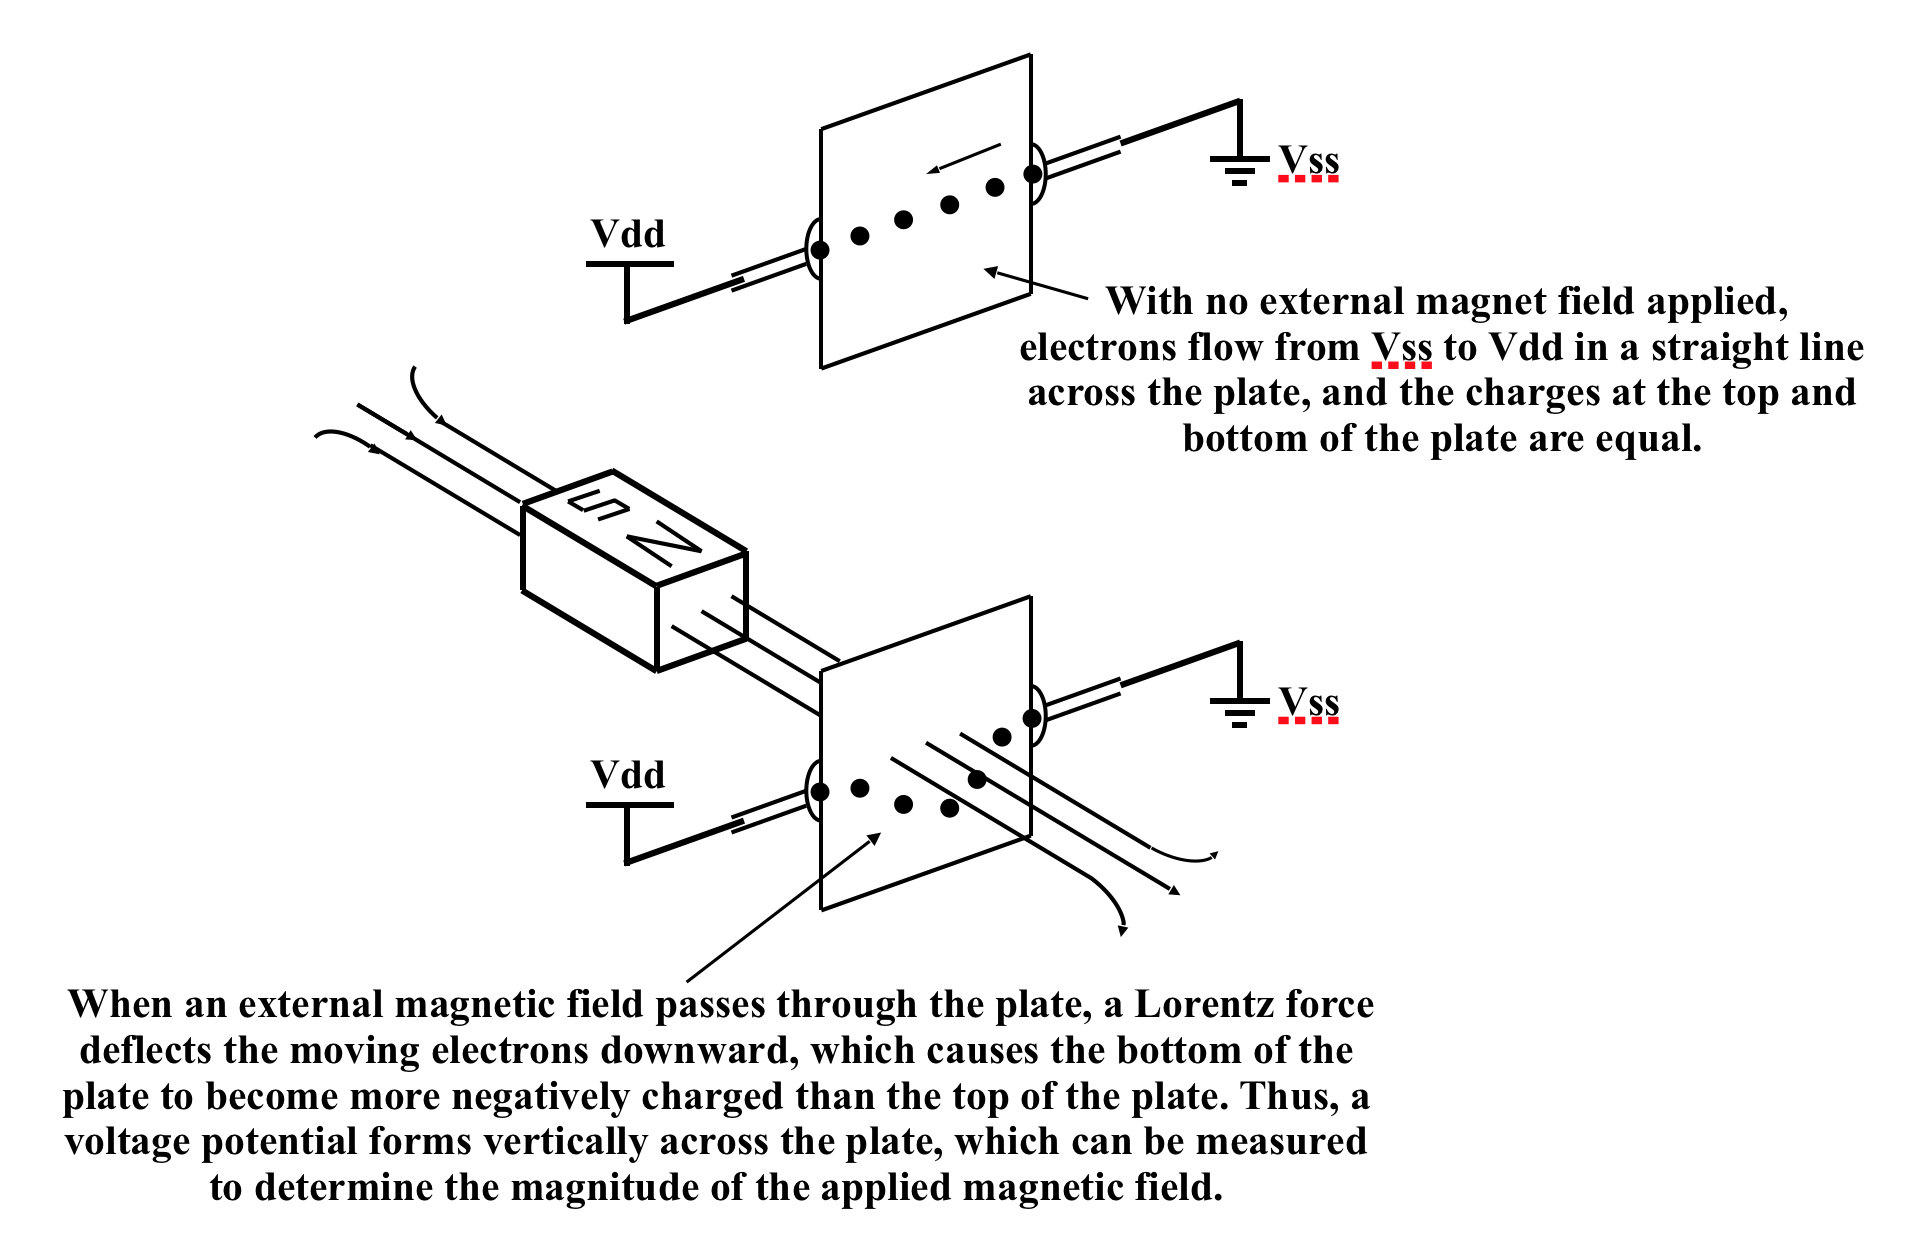
\includegraphics[width=5.5in]{figures/hall_effect}
\caption{Physics of the Hall effect sensor. Stolen shamelessly from Gavin Garner’s Mechatronics manual.}
\label{fig:hall.effect.physics}
\end{center}
\end{figure}
%
%\begin{figure}[htbp]
%\begin{center}
%\includegraphics[width=5.5in]{figures/hall_effect_circuit}
%\caption{Circuit for the Hall effect sensor.}
%\label{fig:hall.effect.circuit}
%\end{center}
%\end{figure}

\subsubsection*{Procedure}

\begin{enumerate}
\item Place your Hall effect sensor in a breadboard and build the circuit shown in the datasheet. Do not connect your Arduino to the breadboard at this time -- use the 5V power supply from your oscilloscope.
\item Place the magnet near the Hall effect sensor and observe Channel 1 on the oscilloscope. Try turning the magnet around and see if the effect is the same.
\item Now turn off the 5V supply and {\bf disconnect the oscilloscope} from the circuit.
\item Connect the Hall effect sensor to your Arduino as you would a button. In fact, you should be able to run your button code from a previous lab and show that you can count the number of times the magnet passes the Hall effect sensor.
\end{enumerate}

{\bf Show your working system to an instructor.}

\vspace{0.25in}
Instructor initials: \rule{2in}{0.4pt}
\vspace{0.25in}

\subsection*{Solenoids}
\label{sec:solenoids}

Solenoids can be used to push or pull things a short distance, and they are commonly applied in electromechanical latch mechanisms. They consist of a ferromagnetic rod that travels through a coil of wire. When the coil is energized, magnetic fields are set up that draw the rod to the center of the coil. Since a solenoid can only move in one direction, springs are often used to return it to its initial position.

\subsubsection*{Procedure}

\begin{enumerate}
\item (This step may be done for you already -- ask before you do this.) Take a piece of cardstock about 8cm x 5cm and roll it into a tube 8cm long and 2 or 3 layers thick. You want it to be stiff enough to allow you to wind wire around it without it collapsing and large enough to allow a nail to slide in and out of it easily.
\item  (This step may be done for you already -- ask before you do this.) Wind a couple hundred turns of electromagnet wire around the tube, leaving a few inches of wire sticking out at each end. Strip the ends like you did before.
\item Place a nail a short distance into the tube and connect the wire ends to a bench top power supply. If the current is high enough (be careful not to overdo it again), the nail will be pulled into the tube. Congratulations -- you’ve just made a solenoid!
\item Examine the datasheet for the solenoid, found on \href{https://www.sparkfun.com/products/11015}{\underline{SparkFun’s product page}}. (If you want to watch the Product Video on that page, go ahead. However, if you ever wire a breadboard like they have in the video, I will kick you out of my class.) How much current does it draw at 5V? What is the maximum duty cycle at 5V?
\item Connect a 12V power supply to the voltage regulator on your experiment board using a barrel jack and adjust the output voltage to 5V by turning the small screw on the blue potentiometer. \item Unplug the 12V supply and screw two wires into the output. Use red for positive and black for negative (ground). Do not strip them more than 1/4” to avoid short circuits. Wire the 5V output through a button and your solenoid, as shown in Figure~\ref{fig:solenoid.circuit}.
\item Plug the 12V supply back in and press the button to activate the solenoid. {\bf Be sure that you do not exceed that maximum on time for the solenoid!} Check the datasheet!
\end{enumerate}

\begin{figure}[htbp]
\begin{center}
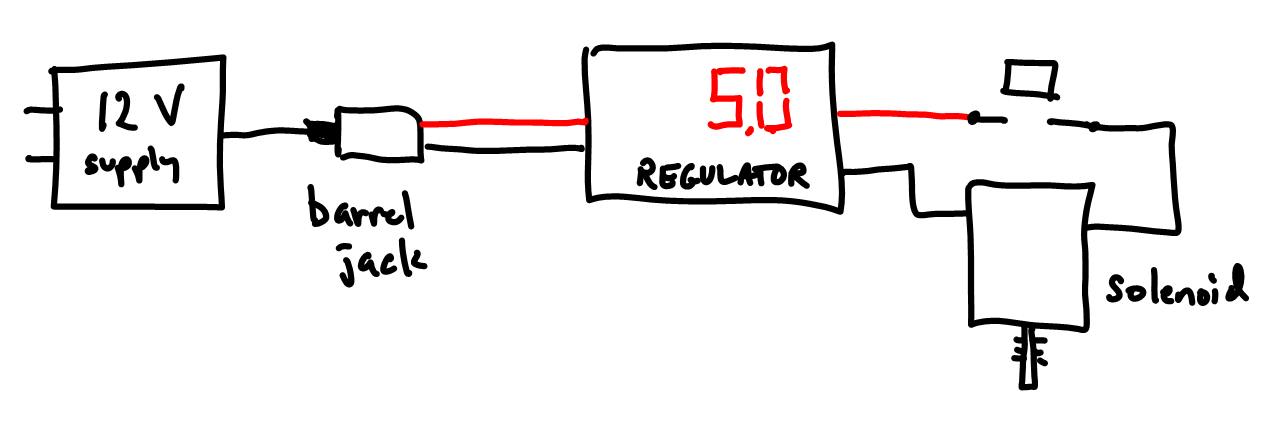
\includegraphics[width=5.5in]{figures/solenoid_circuit}
\caption{Circuit for testing the solenoid.}
\label{fig:solenoid.circuit}
\end{center}
\end{figure}

\subsection*{Relays}

Another application of electromagnetism is found in the electromechanical relay. Here, an electromagnet is used to control a switch, which can be used to drive a much larger current. Figure~\ref{fig:relay.mech} shows a simplified version of the inner workings of such a relay. When the coil is energized, a metal contact switches position to open or close a circuit. Relays are typically used to control very high currents, since it’s easy to make the power side “beefy” enough to handle them.

\begin{figure}
\centering
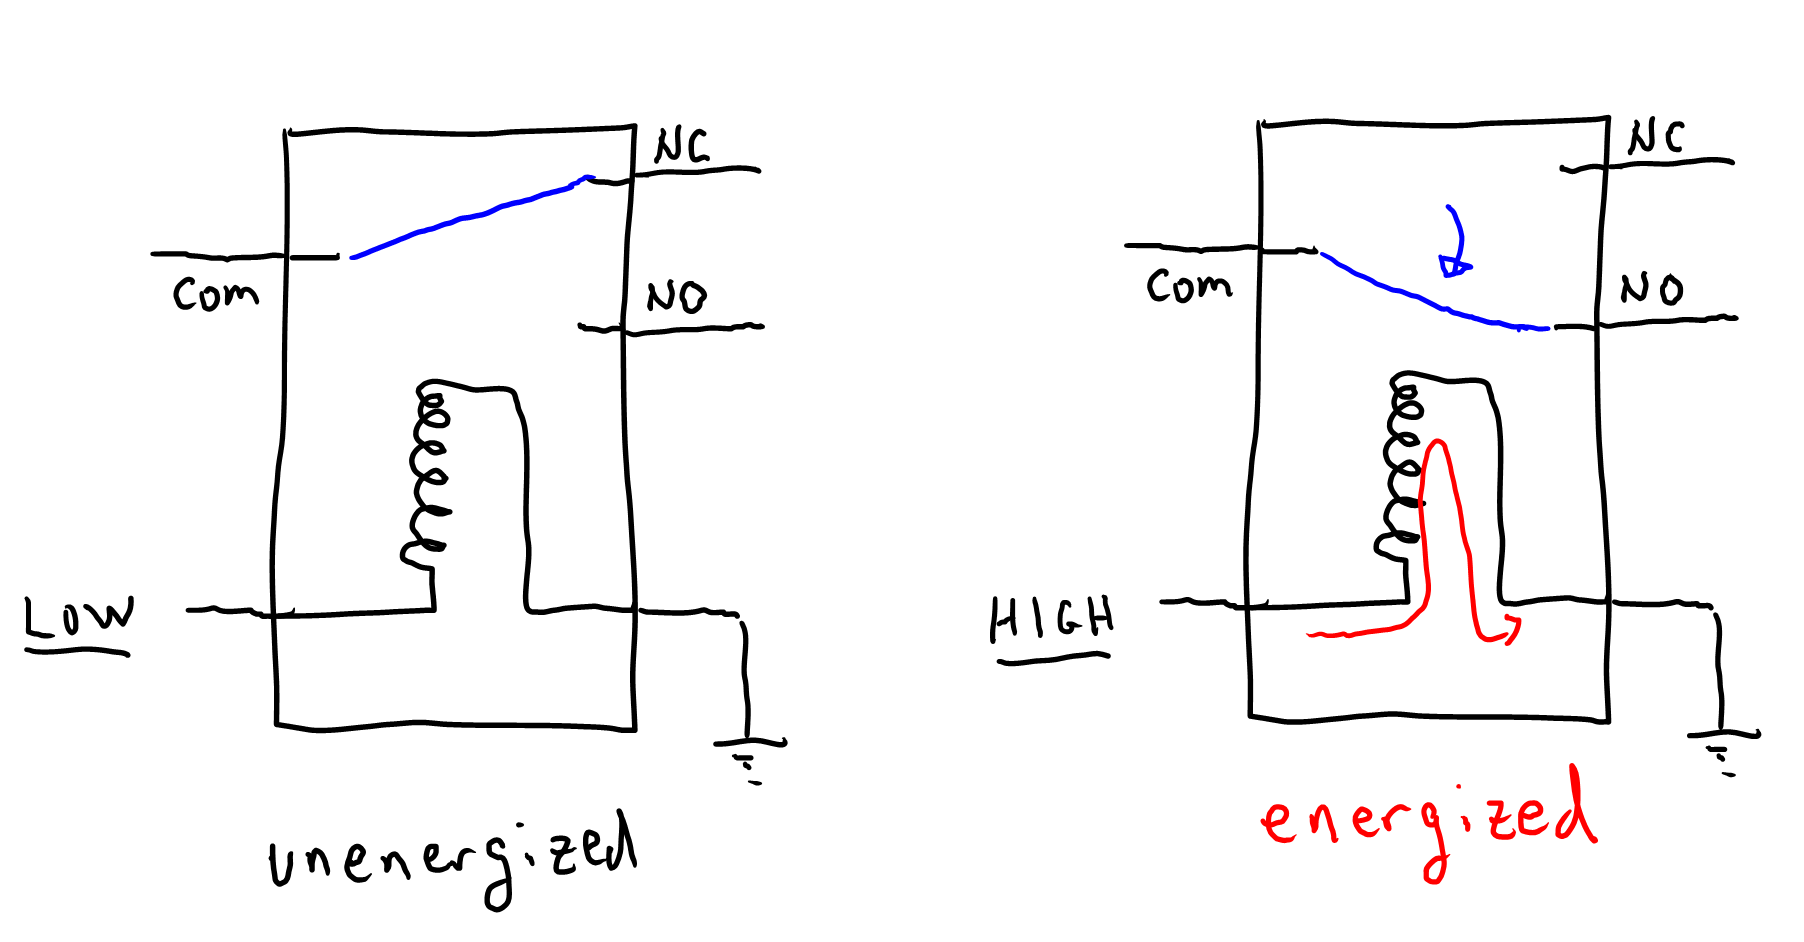
\includegraphics[width=4.5in ]{figures/relay_mech.png}
\caption{Inner workings of a relay. Normally (i.e., when not energized), COM is connected to the normally closed pin (labelled NC). When energized, the connection switches to the normally open (NO) pin.}
\label{fig:relay.mech}
\end{figure}

\begin{enumerate}
\item Do the tutorial in CIRC-11 of the SparkFun tutorials, with modifications:
\begin{itemize}
\item Use the circuit in Figure~\ref{fig:relay}. The one in the tutorial is crap.
\end{itemize}

\begin{figure}
\centering
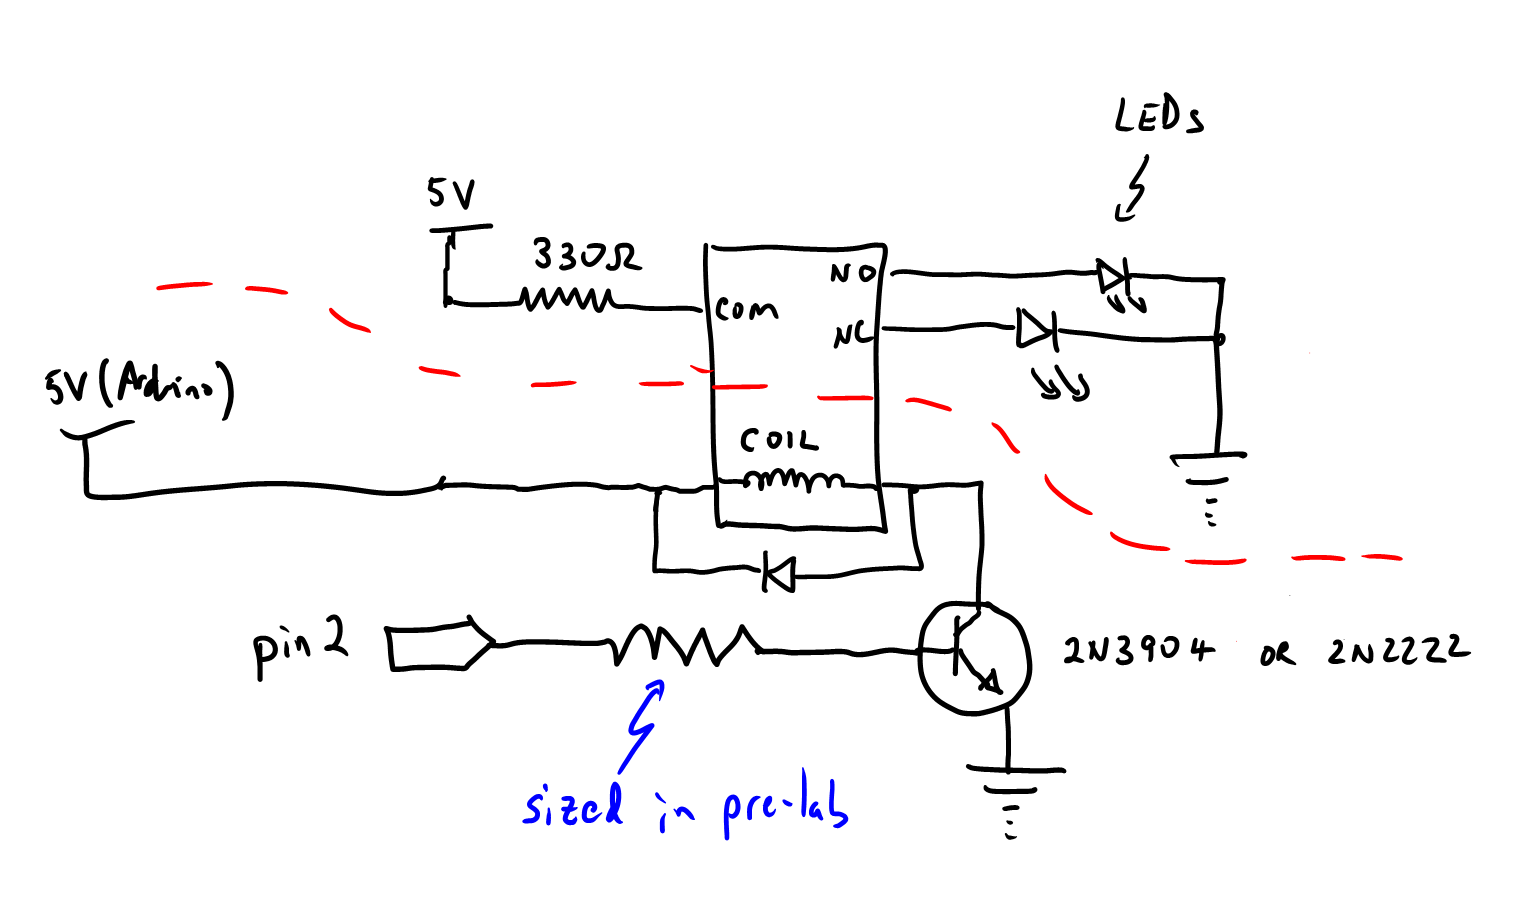
\includegraphics[width=5in ]{figures/relay.png}
\caption{Relay schematic. The dashed line shows the separation between the two circuits, the control circuit on the bottom and the power circuit above.}
\label{fig:relay}
\end{figure}

Some notes:
\begin{itemize}
\item As you have seen in previous labs, the reason we need the transistor is that the relay requires more current than pin 2 can provide. Instead of controlling the relay directly, pin 2 controls the transistor, which then controls the relay, since the transistor can handle a much larger current (this one has a max of 700 mA).
\item The diode -- a `flyback' diode -- is used to ``snub'' a voltage spike whenever the relay turns off. Diodes only pass current in one direction, so when voltage is applied to the relay, all of the current goes through the relay. When the relay opens, energy built up in the coils needs somewhere to go. The diode allows the current drain safely.
\item The relay is an ``SPDT'' relay. The SP stands for ``single pole,'' meaning it has one control input. The DT stands for ``double throw','' meaning that it controls two separate circuits: ``normally open'' and ``normally closed.'' When no voltage applied, the normally closed pin, labelled ``NC’’, is connected to the common pin. That is, “normal” for the relay is no voltage applied, so the normally closed pin is...well...closed. When the relay is energized (voltage applied), the normally open pin, labelled ``NO’’, is connected to the common pin. 
\end{itemize}
\end{enumerate}

\subsection*{RC Servos}

As explained in class, servo motors have circuitry in them that allow you to change the position of the motor by sending a pulse width of a given length. The length of the pulse is kind of a ``code'' that is interpreted by the internal circuitry of the servo, and the length of the low portion can vary somewhat. While controlling the servo is pretty straightforward, it would be a real hassle to generate the pulses yourself. Luckily, the \verb|Servo| library that comes with Arduino does all the heavy lifting for you. For one, it manages the timings using the ATmega's built in timers and interrupts, and it also has code to ensure that you don't drive the servo too far in either direction.
%Arduino has a servo library that allows you to easily send pulses of different lengths; we'll start by doing that ``manually'', and then we'll use the library when we incorporate servos into our systems.

Servo motors are usually rated by \emph{holding torque}. As the term implies, holding torque is the maximum torque that the servo can put out when it's held stationary. To turn, the \emph{load} on the servo must be less than the holding torque, otherwise the motor won't be able overcome the resisting torque. For small, hobbyist motors, typically called \emph{RC servos} because of their popularity in remote control vehicles, holding torque is typically measured in oz.-in.: a motor rated for 1 oz.-in. can provide 1 ounce of force with a moment arm of 1 inch. Doubling the moment arm will halve the force, and vice versa, as I'm sure you recall from your physics courses.

\subsection*{Choosing a motor}

Before we see how the various motors work, we should first wonder why we want to use an RC servo in the first place. The short answer is that RC servos are fairly easy to implement. Really, they are just DC motors with simple feedback circuit all in one convenient package. One could develop similar functionality with a DC motor, some encoders, and a clever control algorithm.\footnote{Your professor did exactly that for Mr. Football's arms during the Tailgate Design Challenge.} For many applications, its ease-of-use makes the RC servo the obvious choice.

On the other hand, for other applications, one often uses a brushed (or brushless) DC motor or a \emph{stepper} motor -- we'll investigate those later in the term. DC motors are typically the cheapest for high-power and high-speed applications, and stepper motors are often used for high-precision applications, though none of these are hard and fast rules. The 3d printers use stepper motors because precision is critical. 

\subsubsection*{Procedure}

\begin{enumerate}
\item Do \emph{Tutorial 8: A Single Servo} in your SIK Guide.
\item Using a potentiometer and the Arduino’s ADC, construct a circuit and program that allows the user to control the position of the servo by turning the potentiometer, such that there is a 1:1 correspondence (e.g., turning the potentiometer clockwise by 45$^o$ will make the servo do the same).
\item Attach the oscilloscope to the servo’s control pin and observe what happens when you turn the potentiometer. How does the Arduino command the servo position?
\end{enumerate}

{\bf Show your working system to an instructor}.

\vspace{0.25in}
Instructor initials: \rule{2in}{0.4pt}
\vspace{0.25in}

\section*{Heating control}

(This section is not complete -- it’ll serve as the challenge for the coming week, but I need to get the lab out sooner, rather than later.)

Your challenge is to implement a heating and cooling system for your greenhouse. Your heating system will compare the actual temperature to a set-point, and turn on the heat if it gets too cold. If it gets too hot, a servo motor will open the top lid to promote passive cooling.

\begin{enumerate}
\item Draw a state diagram that captures the following behavior:
\begin{itemize}
\item Periodically (upon expiration of a timer), the temperature and setpoint are read and compared.
\item When the temperature drops below a minimum (heating) setpoint, the heater turns on.
\item When the  temperature rises above the setpoint, the heater turns off.
\item When the temperature rises above a maximum (cooling) setpoint, the lid opens.
\item When the  temperature falls below the setpoint, the lid closes.
\end{itemize}
\item Use the AD22100 temperature sensor for measuring both the inside and outside temperatures.
\item Draw a block diagram of the system. Show how components connect to each other and the “nature” of that connection (e.g., “5V logic”, “24V power”, etc.
\item Instead of using the Arduino's 5V supply, use your 24V power supply to \emph{independently} supply the \emph{power} (heating) circuit. You will be given 33$\Omega$ power resistors to arrange as you best can to produce maximum heat without exceeding 2A. {\bf Do not make any connections between the 24V circuit and the Arduino system!} Not even ground.
\item Draw a complete schematic of your proposed system using the components you have used up to this point. {\bf Label the connections between components with the voltage and current limits.} For example, The connection from the power supply to the Arduino would have something like, ``$V<12V$'' (the Arduino's limits), and, ``$I < 2A$'' (the power supply's limits).Show the schematic to an instructor.
\item Implement the system with the power resistors and your IKEA greenhouse. \emph{Use event-driven programming.}
\item Add code to print both the setpoint and the current temperature to the serial monitor. Set the timer so that the sensors are read every 5 seconds. You may \emph{not} use \verb|delay()|.
\item Demonstrate your working system to an instructor. The instructor will also inspect your code.
\end{enumerate}

\subsection*{Hysteresis}

The system you developed in the previous section still has a minor flaw, namely that noise in the temperature sensing can lead to the relay switching on and off rapidly. In a full-sized heating system (e.g., a residential furnace), such \emph{short-cycling} can lead to unnecessary wear and tear on the system; in ours, it could theoretically lead to premature failure of the relay. It's only a \$1 relay, but still, we'd like to avoid the behavior.

As described in the reading, one way to combat this is to use \emph{hysteresis}, or memory, which allows us to change our behavior based on past events. For the system at hand, you will add a variable that raises or lowers the nominal set-point, depending on whether we've received a call for heat or cooling. 

\begin{enumerate}
\item Implement a 1C hysteresis band. Make the band ``below'' the set-points. That is, the heater should come on when the temperature drops to 1C below set-point, and turn off when set-point is reached. Be sure to update your state transition diagram, which will make the programming task almost trivial.
\item Demonstrate your working system to an instructor.
\end{enumerate}


\end{document}

\clearpage

\section{Pre-lab}
\label{sec:prelab}
{\bf This is an individual assignment!}
\emph{Answers with incomplete or incorrect units will be marked as wrong!}
\begin{enumerate}
\item In theory, if the number of coils around an electromagnet is doubled, how will that affect the force exerted by that magnet, assuming the current remains the same?
\vspace{0.5in}
\item What if the current is doubled, \emph{ceteris paribus}?
\vspace{0.5in}
\item Do Problem 24.3(a) in Carryer \emph{et al.}.
\vspace{2in}
\item Read Problem 24.6 in Carryer \emph{et al.}. We’ll work through it in class on Wednesday.
\end{enumerate}
